\section{Results}

Each \Cyclus result is shown as a bar, and the excel solution in the
paper is shown as a line, for better visualization. The results are
simply a reproduction of the plots displayed in the paper. The excel
results are obtained by personal contact with the paper author
Bo Feng at Argonne National Laboratory.


\begin{figure}[htbp!]
	\begin{center}
		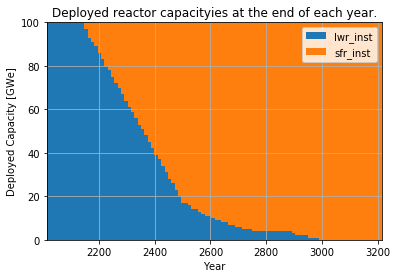
\includegraphics[scale=0.6]{./images/results/power_plot.png}
	\end{center}
        \caption{Deployed reactor capacities at the end of each year.}
	\label{fig:pow_plot}
\end{figure}



\begin{figure}[htbp!]
	\begin{center}
		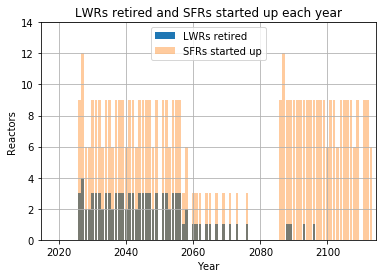
\includegraphics[scale=0.6]{./images/results/dep.png}
	\end{center}
        \caption{\glspl{LWR} retired and \glspl{SFR} started up each year.}
	\label{fig:dep}
\end{figure}

%%%%%%%%%%%%%%%%%%%%%% DON'T HAVE THE PICTURE YET
\iffalse
\begin{figure}[htbp!]
	\begin{center}
		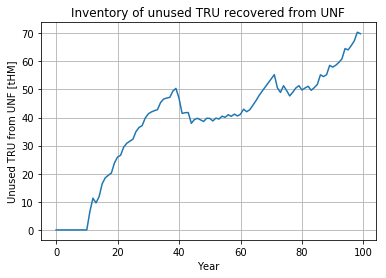
\includegraphics[scale=0.6]{./images/results/tru.png}
	\end{center}
        \caption{Inventory of unused \gls{TRU} recovered from \gls{UNF}.}
	\label{fig:tru}
\end{figure}
\fi


The annual fuel loading rates are shown in table \ref{fig:fuel_load_unfixed}.
The spike is due to the initial core loading of the 100 reactors that were
deployed in time first timestep. If we set the first two datasets equal to
the third point (fuel loaded at 2017), we get the same plot as the verification
study results (shown in table \ref{fig:fuel_load}).


\begin{figure}[htbp!]
	\begin{center}
		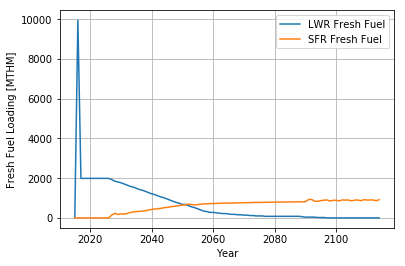
\includegraphics[scale=0.6]{./images/results/fuel_load_unfixed.png}
	\end{center}
        \caption{Annual fresh fuel loading rates (first cores and reload fuel).
        		 The initial spike is due to the first core fuel loading of reactors
        		 since they are all assumed to be deployed at 2016.}
	\label{fig:fuel_load_unfixed}
\end{figure}


\begin{figure}[htbp!]
	\begin{center}
		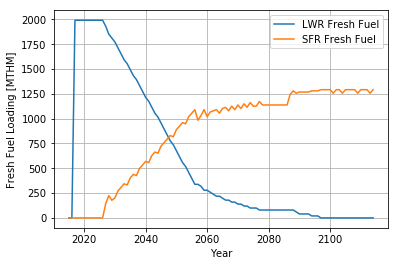
\includegraphics[scale=0.6]{./images/results/fuel_load.png}
	\end{center}
        \caption{Annual fresh fuel loading rates (first cores and reload fuel).}
	\label{fig:fuel_load}
\end{figure}



\begin{figure}[htbp!]
	\begin{center}
		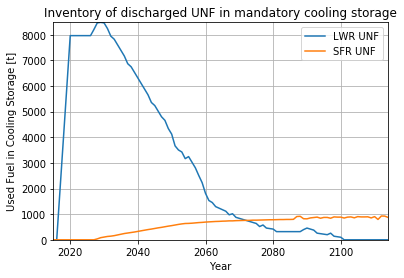
\includegraphics[scale=0.6]{./images/results/fuel_discharge.png}
	\end{center}
        \caption{Inventory of discharged \gls{UNF} in mandatory cooling storage.}
	\label{fig:fuel_discharge}
\end{figure}



\begin{figure}[htbp!]
	\begin{center}
		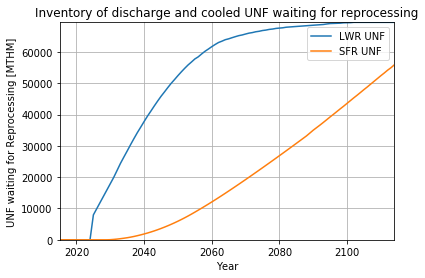
\includegraphics[scale=0.6]{./images/results/waiting.png}
	\end{center}
        \caption{Inventory of discharged and cooled \gls{UNF} waiting for reprocessing}
	\label{fig:waiting}
\end{figure}


\begin{figure}[htbp!]
	\begin{center}
		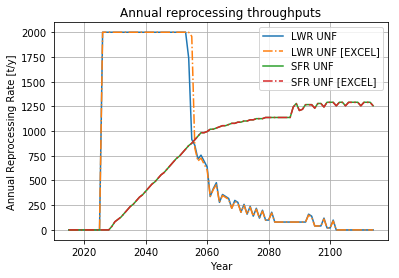
\includegraphics[scale=0.6]{./images/results/rep.png}
	\end{center}
        \caption{Annual reprocessing throughputs.}
	\label{fig:rep}
\end{figure}

